\documentclass[a4paper,10pt]{article}
\usepackage[left=3cm,top=3cm,right=3cm,bottom=3cm,head=4cm,includefoot]{geometry}

%%%%%%%%%%%%%%%%%%%%%%%%%%%%%%%%%%%%%%%%%%%%%%%%%%%%%%%%%%%%%%%%%%%%%%%%
% Paquetes utilizados
%%%%%%%%%%%%%%%%%%%%%%%%%%%%%%%%%%%%%%%%%%%%%%%%%%%%%%%%%%%%%%%%%%%%%%%%

% Graficos complejos
\usepackage{graphicx}
\usepackage{rotating}
\usepackage{caption}
\usepackage{subcaption}
\usepackage{placeins}

% Soporte para el lenguaje español
\usepackage{textcomp}
\usepackage[utf8]{inputenc}
\usepackage[T1]{fontenc}
\DeclareUnicodeCharacter{B0}{\textdegree}
\usepackage[spanish]{babel}

% Codigo fuente embebido
\usepackage{listings}

% PDFs embebidos para el apendice
\usepackage{pdfpages}

% Matematicos
\usepackage{amssymb,amsmath}

% Tablas complejas
\usepackage{multirow}

% Formato de parrafo
\setlength{\parskip}{1ex plus 0.5ex minus 0.2ex}

%%%%%%%%%%%%%%%%%%%%%%%%%%%%%%%%%%%%%%%%%%%%%%%%%%%%%%%%%%%%%%%%%%%%%%%%
% Titulo
%%%%%%%%%%%%%%%%%%%%%%%%%%%%%%%%%%%%%%%%%%%%%%%%%%%%%%%%%%%%%%%%%%%%%%%%

% Titulo principal del documento.
\title{\textbf{Trabajo Practico 2: Personas}}

% Informacion sobre los autores.
\author{\\
  Arana Andrés, \textit{P. 86.203}                                 \\
  \texttt{and2arana@gmail.com}                                     \\ [2.5ex]
  Arias Damián, \textit{P. 89.952}                                 \\
  \texttt{arias.damian@gmail.com}                                  \\ [2.5ex]
  Sergio Matias Piano, \textit{P. 85.191}                          \\
  \texttt{smpiano@gmail.com}                                       \\ [2.5ex]
                                                                   \\
  \normalsize{2do. Cuatrimestre de 2014}                           \\
  \normalsize{75.59 Técnicas de Programación Concurrente 1}        \\
  \normalsize{Facultad de Ingenieria, Universidad de Buenos Aires} \\
}
\date{}

%%%%%%%%%%%%%%%%%%%%%%%%%%%%%%%%%%%%%%%%%%%%%%%%%%%%%%%%%%%%%%%%%%%%%%%%
% Documento
%%%%%%%%%%%%%%%%%%%%%%%%%%%%%%%%%%%%%%%%%%%%%%%%%%%%%%%%%%%%%%%%%%%%%%%%

\begin{document}

% ----------------------------------------------------------------------
% Top matter
% ----------------------------------------------------------------------
\thispagestyle{empty}
\maketitle

\begin{abstract}

  Este informe sumariza el desarrollo del trabajo practico 2 de la materia
  Técnicas de Programación Concurrente I (75.59) dictada en el segundo
  cuatrimestre de 2014 en la Facultad de Ingenieria de la Universidad de Buenos
  Aires. El mismo consiste en la construccion de una aplicación de gestión de
  información de contacto de personas compuesta por un servidor de datos y
  varios clientes conectados a través de una cola de mensajes.

\end{abstract}

\clearpage

% ----------------------------------------------------------------------
% Indice
% ----------------------------------------------------------------------
\tableofcontents
\clearpage


% ----------------------------------------------------------------------
% Desarrollo
% ----------------------------------------------------------------------
%\part{parte}


\section{Análisis del problema}

\subsection{Descripción}

\section{Hipótesis}

\clearpage
\section{Desarrollo de la solución}

\clearpage
\section{Uso de la aplicación}

\clearpage
\section{Diagramas}
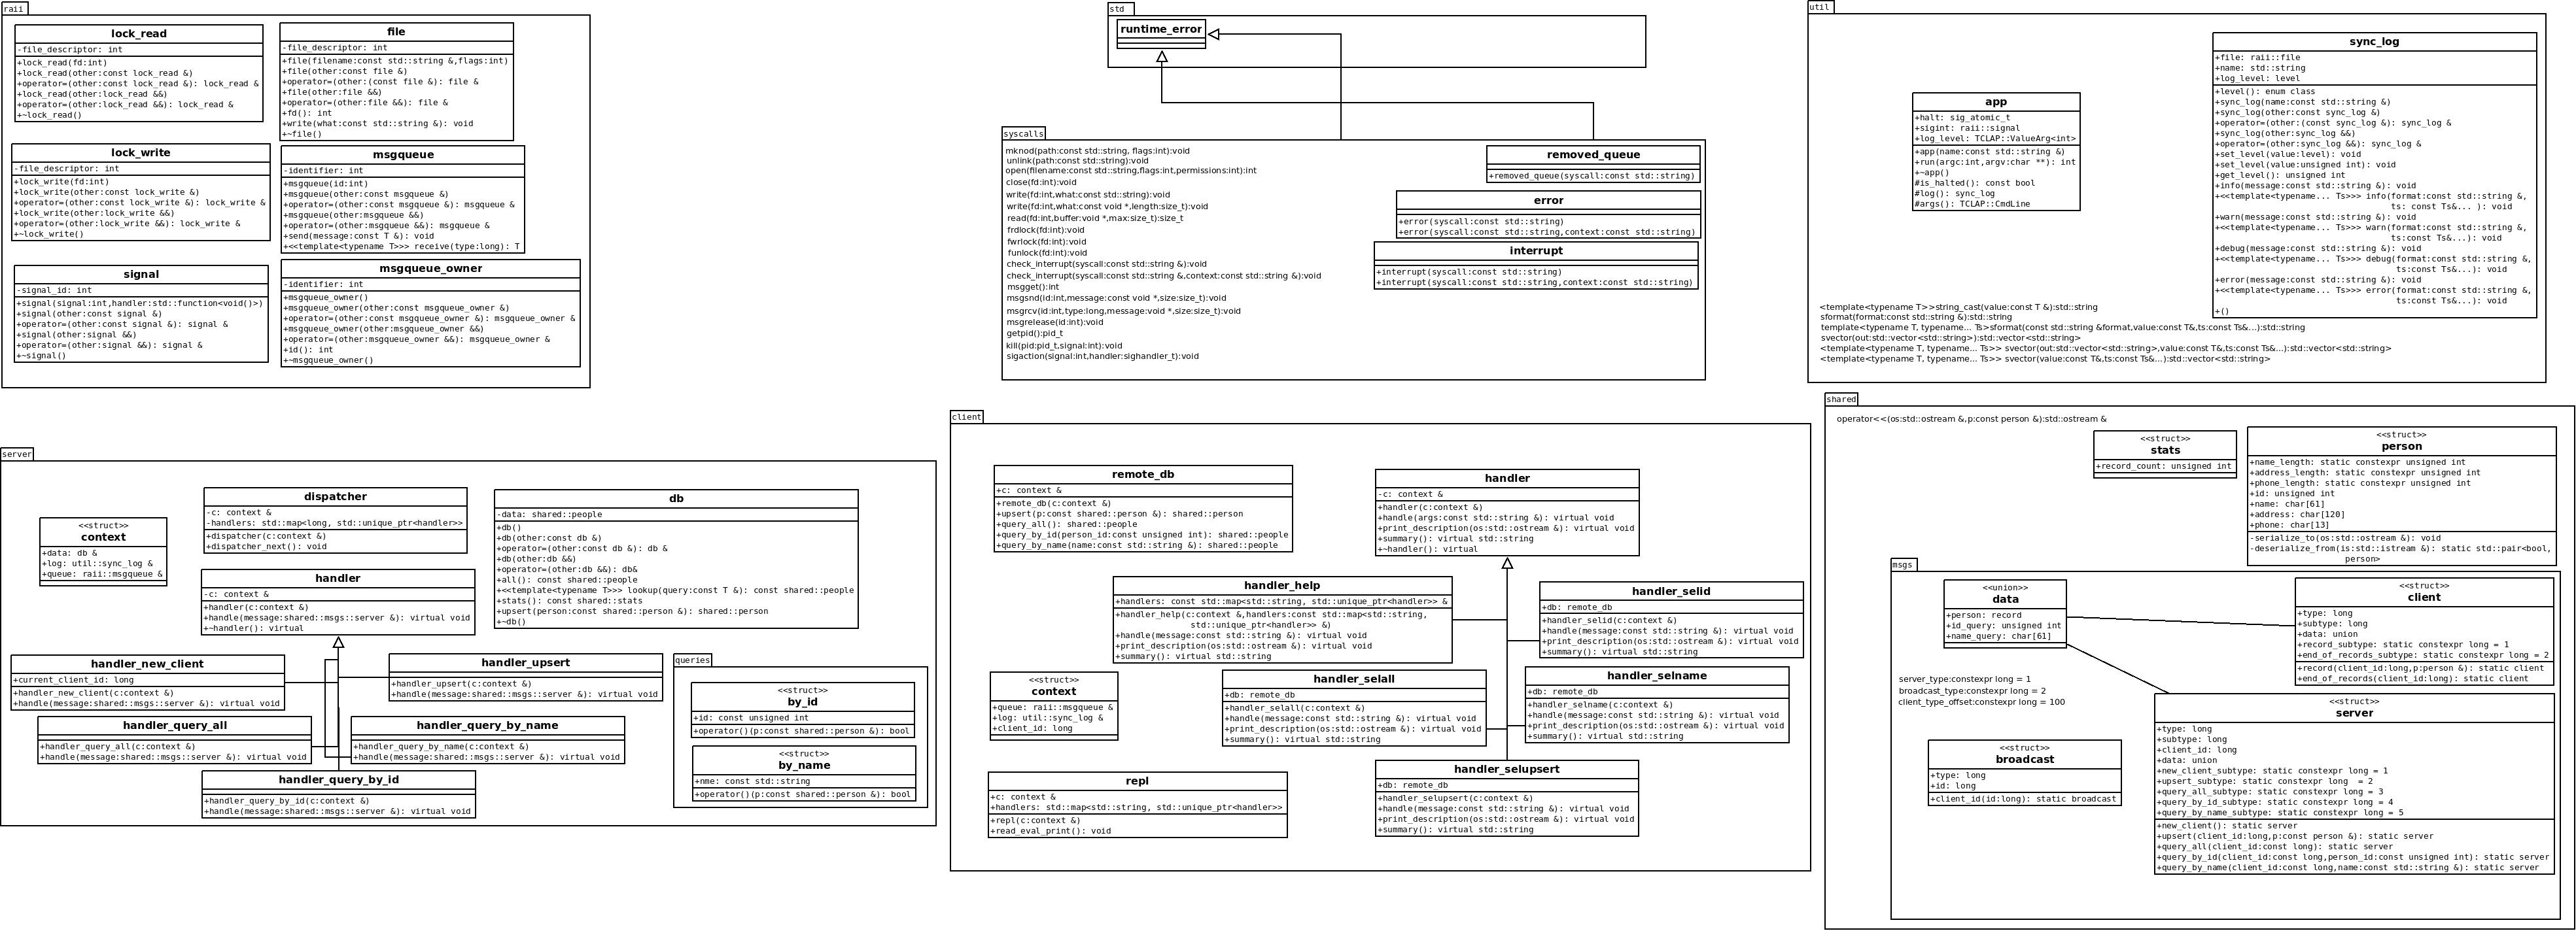
\includegraphics[width=23.5cm, height=15cm, angle=90]{build/doc/diagrams/classes_diagram.png}

\clearpage
\section{Enunciado}
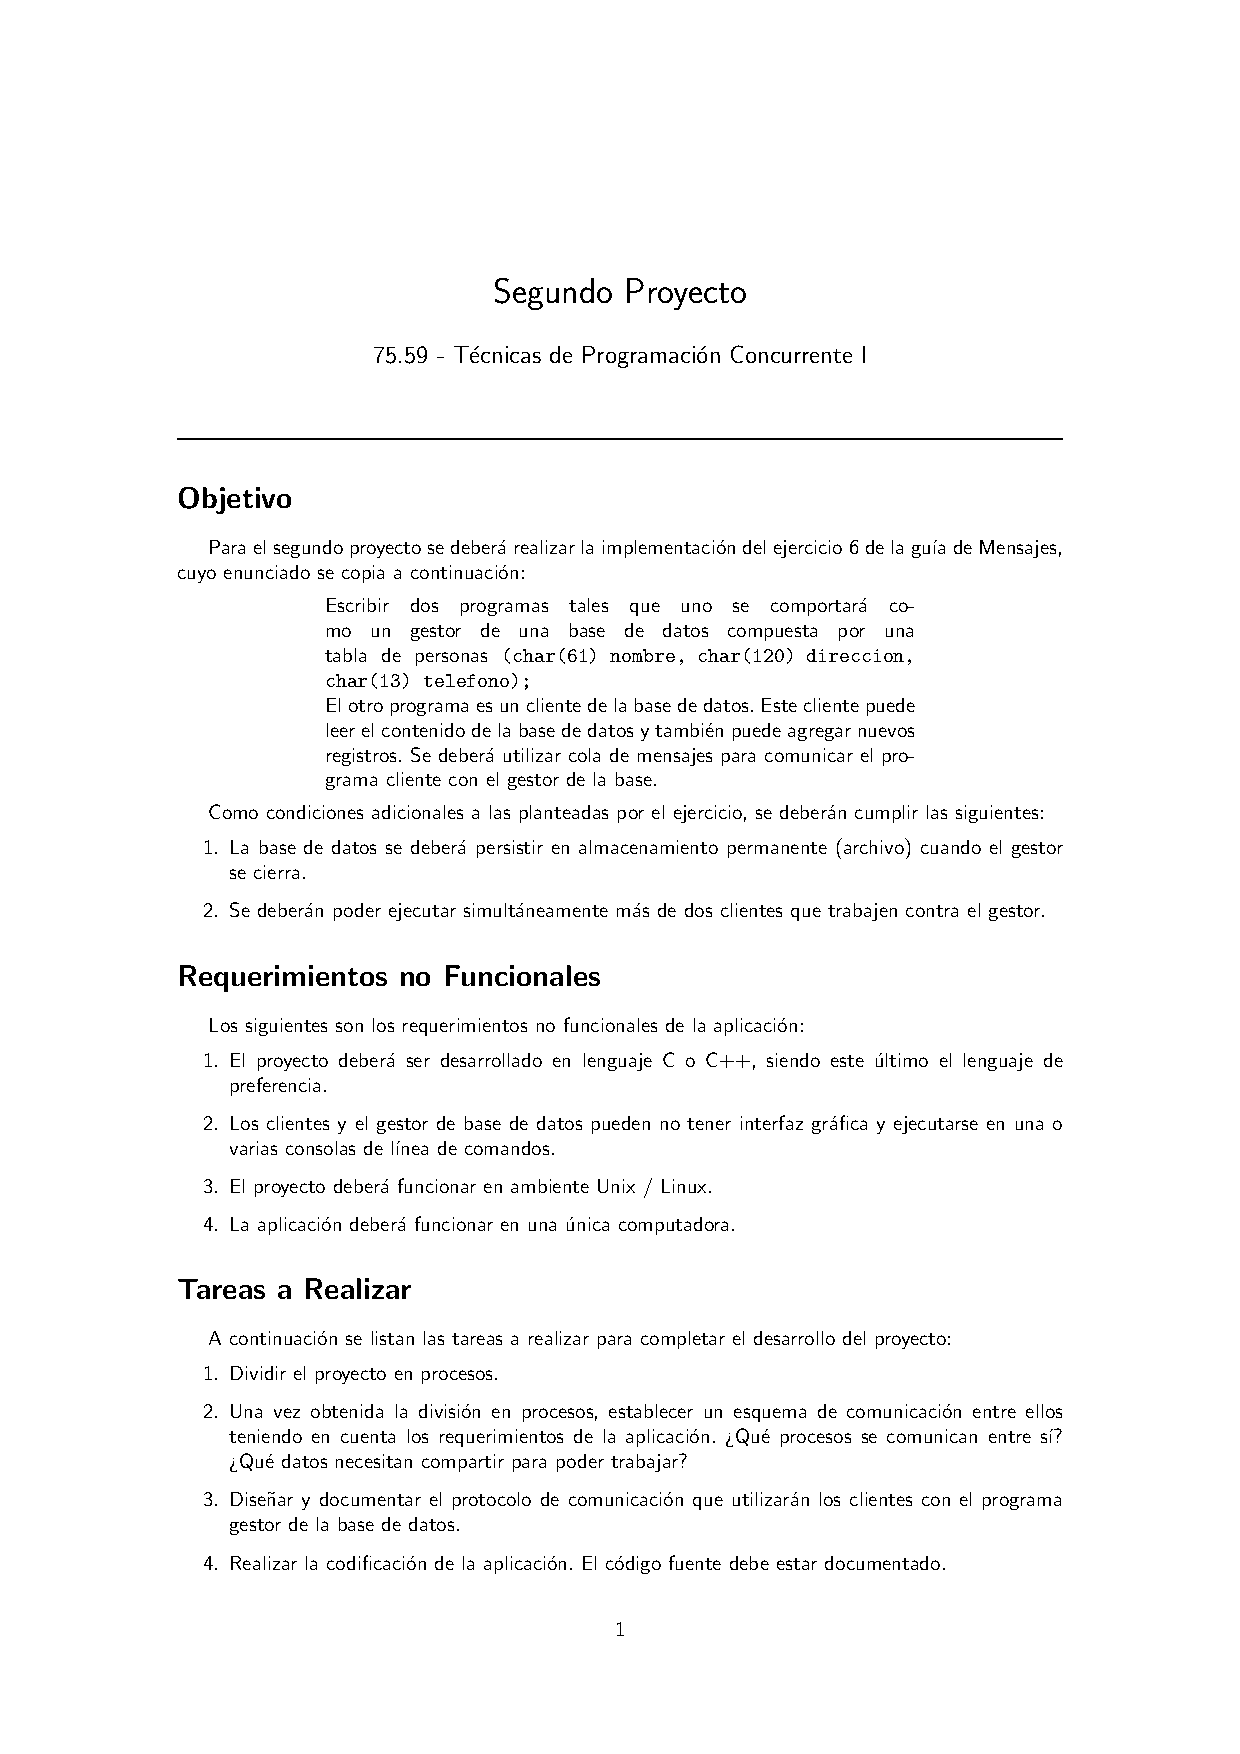
\includepdf[pages={-}]{enunciado.pdf}

\end{document}
